\chapter{Introduction}\label{ch:introduction}

\section{Outflows from BNS Mergers}\label{sec:bns}
    Due to the joint electromagnetic and gravitational wave detection of the binary
    neutron star merger event GW1701817 (see \cite{abbott_2018}), there has
    been renewed interest in SGRBs.  Specifically, this detection gives credence to the
    claim that the central engines of SGRBs are binary neutron star mergers (see
    \cite{narayan_1992}). However, there are other aspects of the process that
    are not as clear. Specifically, several aspects of GW170817 have not been completely
    explained. The main concerns are as follows (\cite{lazzati_2020}):

    \begin{itemize}

        \item The outflow of GRB170817A was lower in energy than a typical cosmological
            SGRB, by a factor of $10^4 - 10^5$, even though the event was one of the
            closest GW events recorded, at a distance of $\sim$ 40 Mpc. This could be
            due to two factors :

            \begin{itemize}

                \item The structured jet was off-axis with respect to the observer.

                \item The internal engine powering this SGRB was intrinsically less
                    energetic, and differs from the one observed in other typical SGRBs.

            \end{itemize}

        \item A clear consensus has not been reached on how the gamma-ray prompt
            emission was produced. The uncertainty partly comes from the fact that the
            various delays involved before the prompt emission is observed are not
            accurately constrained. Models which have been considered include :

            \begin{itemize}

                \item The structured outflow model, characterised by functions for the
                    Lorentz factor and the energy per unit solid angle, both of which
                    vary with the angle made with the polar jet axis ($\theta$). This
                    model produces detectable signals even at moderately large off-axis
                    angles.

                \item The shock breakout model, wherein the leading edge of the wind
                    emits the prompt emission as it breaks out of the cocoon of nuclear
                    matter ejected before the jet was launched. This model has been
                    shown to explain the energetics and spectrum of the prompt emission,
                    although it does require a setup in which the wind is fast enough so
                    that it can reach a large enough distance at breakout.

            \end{itemize}

    \end{itemize}

    More light can be shed on these questions by observing more such SGRBs, using both
    the gravitational wave (GW) and electromagnetic (EM) windows.  However, the
    possibility of joint detections are slim, due to the fact that the EM observations
    are highly dependent on the viewing angle of the system with respect to the observer
    (due to relativistic beaming), whereas GW signal amplitudes depend on the distance
    to the event (see ).\\
    Given that this is the case, it would be expedient to look for constraints on the
    structure parameters of various models.  Furthermore, it would be useful to develop
    models which are resilient to non-detections, and can produce constraints on the
    parameters using even upper limits on the flux/fluence observed by the various EM
    follow-up satellites, such as INTEGRAL, Fermi or Swift.\\

    \subsection{Modelling outflows from BNS Mergers}\label{ssec:bns-outflows}

    As mentioned before, the electromagnetic follow-up of the binary neutron star merger
    event GW170817 helped measure the various time delays between the time of the GW
    signal trigger (which roughly is the merger time itself) and the time the gamma-ray
    signals were picked up. This time delay is denoted $\Delta t_{GW-\gamma}$, and was
    around 1.75 seconds for this event.  The components which make up this delay are as
    follows (\cite{lazzati_2020}):

    \begin{itemize}

        \item \textbf{Engine Delay} -- this is the delay due to a transition mechanism
            in the central engine which powers the jet (such as a metastable, fast
            spinning neutron star collapsing into a black hole when its rotation period
            increases; this process can take years) or due to the time elapsed in
            amplifying the magnetic field to a value large enough for jet launching
            (this process is significantly faster, taking only seconds). This is denoted
            by $\Delta t_{eng}$.

        \item \textbf{Wind Delay} -- this is simply a delay in the launching of a
            non-relativistic wind due to the neutron-rich matter from the progenitor(s)
            being tidally shredded. For this reason, it can be \textit{negative} as
            well, since the tidal shredding can occur before the merger itself. This is
            denoted as $\Delta t_{wind}$.

        \item \textbf{Breakout Delay} -- if the wind is ejected before the jet, then the
            latter will have to propagate through the former. This happens at a
            sub-relativistic speed, whereas the GW signal travels at a relativistic
            speed. The delay due to this crossing is the breakout delay, and is denoted
            $\Delta t_{bo}$. During this time, jet-wind interactions cause the
            development of a structured outflow that maintains a bright core but also
            has energetic wings at large polar angles.

        \item \textbf{Photospheric Delay} --  once the jet has crossed the wind, it
            still needs to propagate out to the photospheric radius, where the outflow
            becomes transparent and the prompt gamma-ray emission is radiated. The delay
            from the breakout radius to the photospheric radius is $\Delta t_{ph}$. This
            is given by (for GW170817):

            \begin{equation}
                \label{eq:4}
                \Delta t_{ph} \sim \dfrac{R_{ph}}{c \Gamma^2} =
                    1.4 \dfrac{R_{ph}}{2 \times 10^{12} \text{ cm}}
                    \left( \dfrac{7} {\Gamma} \right)^2 \text{ s}
            \end{equation}

        \item \textbf{Dissipation Delay} -- this is a requirement in some models, such
            as the internal shock synchrotron model, wherein the outflow needs to travel
            to the internal shock radius before the bulk energy of the flow is
            dissipated and turned into radiation. The time required to get to this point
            after crossing the photospheric radius is the dissipation delay, denoted
            $\Delta t_{\gamma}$

    \end{itemize}

    Several attempts to constrain the various time delay components have been made.
    However, except for relative comparisons, no conclusions have been arrived upon.
    For example, one can only say that the photospheric delay is the major component out
    of all the delays, and that wind delay (if non-zero) has to be lesser than the jet
    delay, so that the jet catches up to the wind and the jet-wind interaction generates
    the structured outflow. Fig. \ref{fig:jet_delay} summarises these delays in the
    broader context.

    \begin{figure}[H]
        \centering
        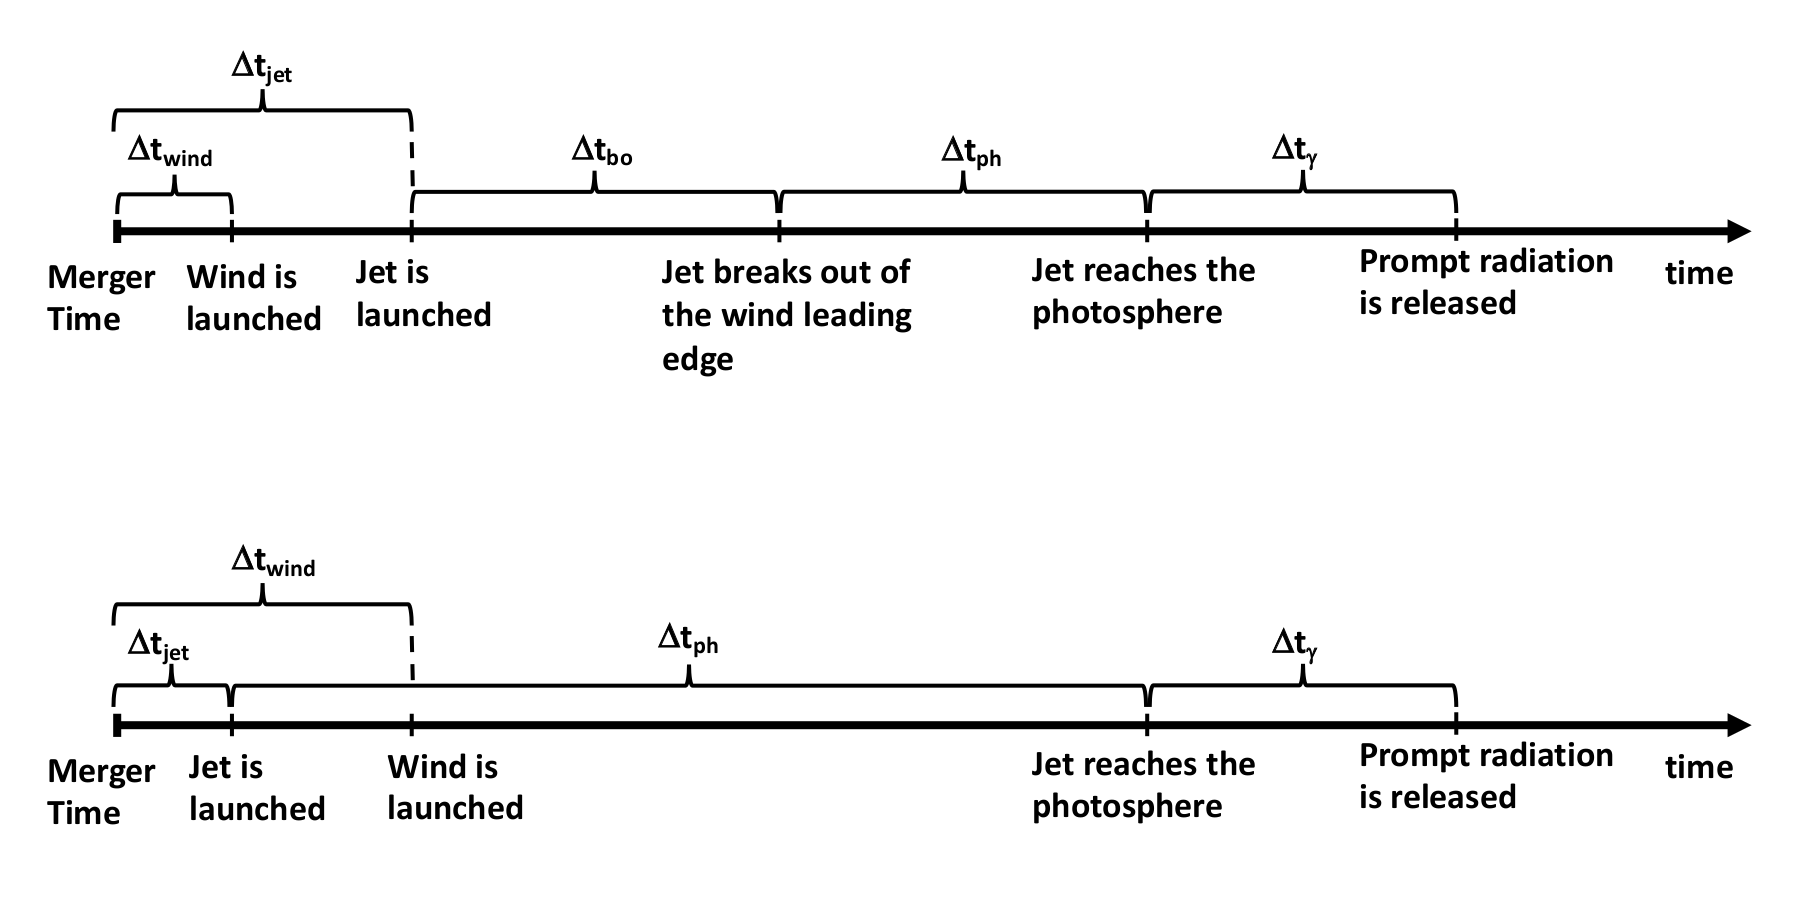
\includegraphics[width=12cm]{jet_delay}
        \caption[Relative Positions of Jet Delays]
             {
                    Two possible scenarios for the relative positioning of the delays in
                    time, which contribute to $\Delta t_{GW-\gamma}$.  Owing to the
                    requirement of a structured outflow, GW170817 possibly follows the
                    top timeline. The relative contributions of the various delays are
                    debated, but it is agreed that $\Delta t_{wind} < \Delta t_{jet} \ll
                    1$ s, $\Delta t_{bo} \ll 1$ s, $\Delta t_{\gamma} \sim 0$ and
                    $\Delta t_{ph} \sim \Delta t_{GW-\gamma}$.
             }
        \label{fig:jet_delay}
    \end{figure}

    Due to the uncertainties in the delay terms, several models for the jet can explain
    the energetics and observed structure. Numerical simulations are also unequivocal
    about their favouring of one model over the other (see \cite{shibata_2019}).
    Some models try to explain the \textit{apparent} structure of the jet, which are the
    observables seen by a particular observer at a particular viewing angle. Other
    models are used to explain the \textit{intrinsic} structure, such as the polar angle
    variation of the bulk Lorentz factor and the energy across the solid angle, in the
    jet co-moving frame. See \cite{salafia_2015} for a detailed discussion of
    the differences between the two structures. Some of the models considered are
    described below (see also Figs. \ref{fig:tophat} and \ref{fig:jet_models}):

    \begin{itemize}

        \item Top-hat -- This model, as used in \cite{saleem_2020B}, assumes
            that the bulk Lorentz and energy functions drop to zero beyond some cutoff
            angle, $\theta_j$. Below this threshold, the functions are at their
            respective on-axis values.

       \item Gaussian -- This model is widely used, in some contexts to explain the
           apparent jet structure (by \cite{hayes_2020}), and in others the
           intrinsic jet structure (by \cite{saleem_2020B}). The former is
           simply given by $y_{GJ}(\theta) = e^{- \frac{1}{2} \left(
           \frac{\theta}{\theta_{\sigma}} \right)^2}$, since the authors consider only
           the apparent jet structure, as explained above and $\theta_\sigma$ is a
           structure parameter which is inferred by the authors' Bayesian inference.\\
           In the latter, as the authors consider the intrinsic jet structure, they
           assume that $\Gamma \beta (\theta) = \Gamma_0 \beta_0 \exp\left(- \theta^2 /
           2\theta_c^2\right)$ and that $\epsilon (\theta) \propto \exp(- \theta^2 /
           \theta_c^2)$\footnote{
               This is the normalised energy profile function.  The normalisation
               constant is estimated by the condition $2\pi \int d(\cos \theta)
               \epsilon(\theta) = E_{tot., \gamma}$, where $E_{tot., \gamma}$ is the
               total energy in gamma-rays.
           }, and derive the observed properties (see below).

        \item Power Law -- This model is used by \cite{hayes_2020} to explain
            the apparent structure of the jet, assuming that any variation in the energy
            is simply because of relativistic beaming and the jet being viewed off-axis.
            It is given using the shape function $y(\theta)$ (which is multiplied with
            the on-axis isotropic equivalent energy $E_{iso, 0}$ to give
            $E_{iso}(\theta)$\footnote{Using the equation $E_{iso}(\theta_v) = E_{iso,
            0} \cdot y(\theta_v)$}):

                \begin{equation}
                    \label{eq:5}
                    y(\theta) = \begin{cases}
                                    1,
                                        & 0 \leq \theta \leq \theta_c, \\
                                    (\theta/\theta_c)^{-2},
                                        & \theta_c < \theta \leq \theta, \\
                                    0,
                                        & \theta_j < \theta
                                \end{cases}
                \end{equation}
                Here $\theta_c$ and $\theta_j$ are simply structure parameters, inferred
                using Bayesian methods.

    \end{itemize}

    \begin{figure}[H]
        \centering
        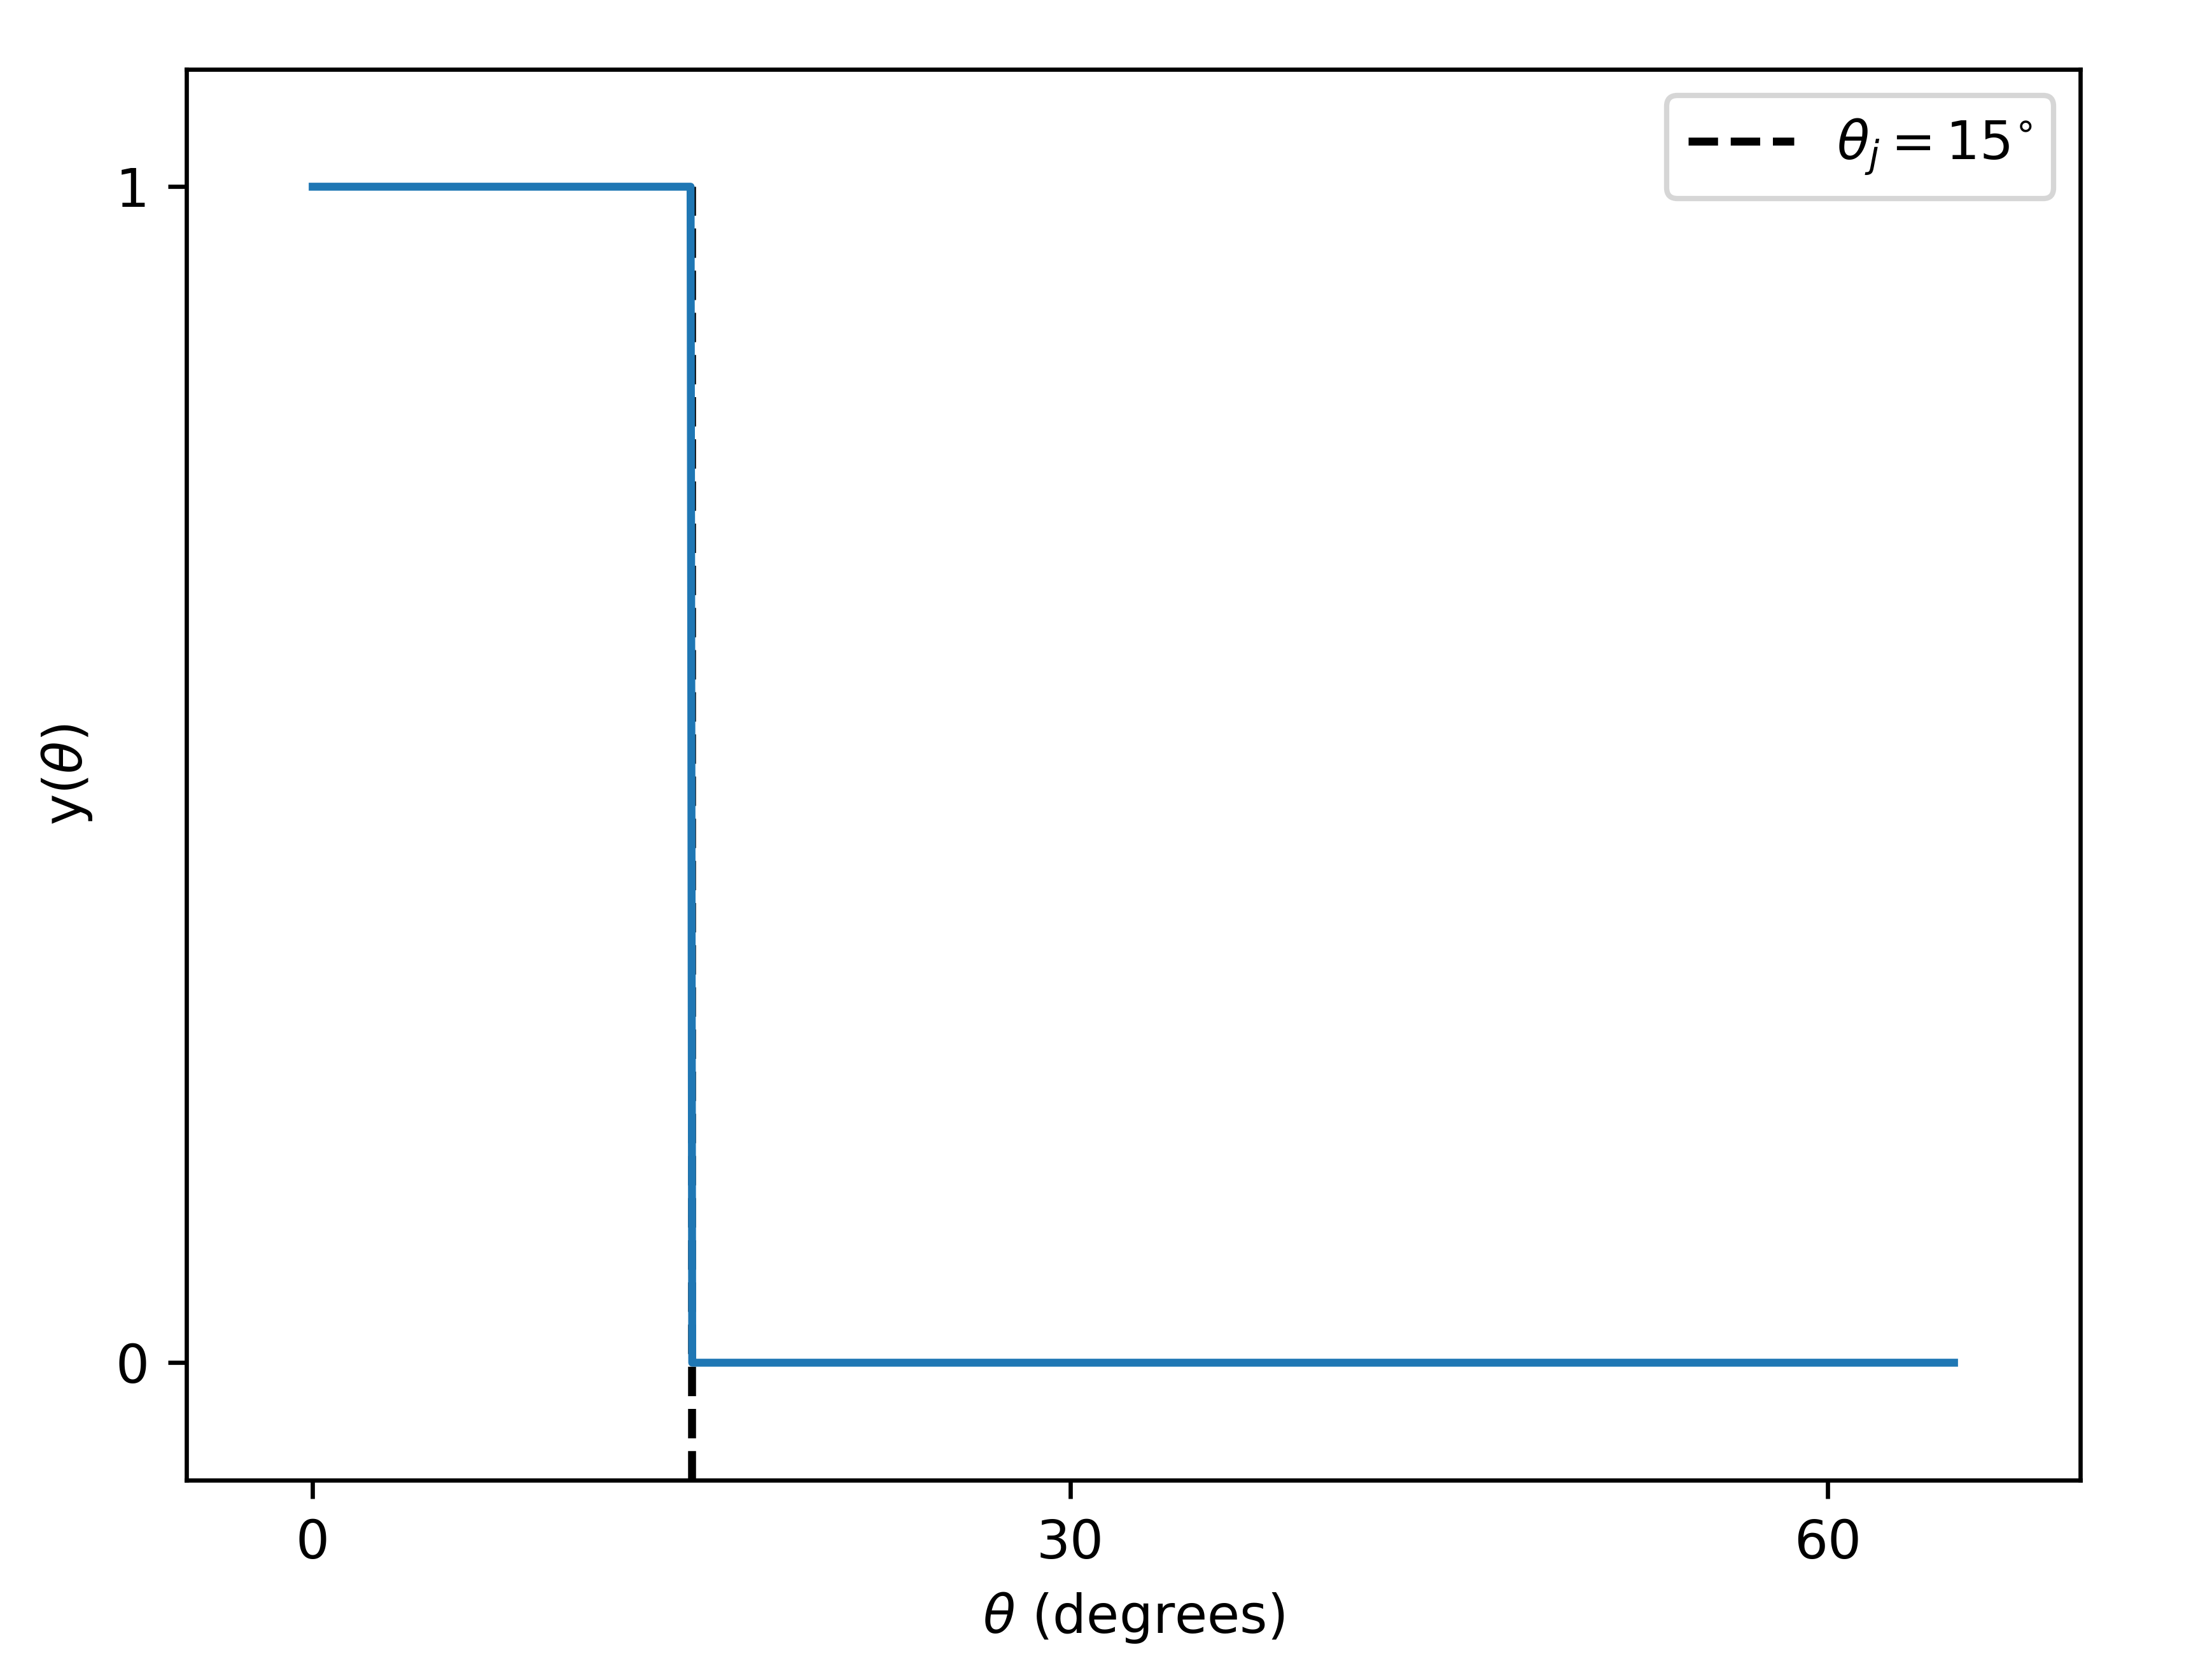
\includegraphics[width=10cm]{tophat}
        \caption[Tophat jet structure model]{
                    Functional form of the tophat jet structure model, as considered in
                    \cite{saleem_2020B}. The dashed line denotes the jet angle
                    $\theta_j = 15^{\circ}$.
             }
        \label{fig:tophat}
    \end{figure}

    \begin{figure}[H]
        \centering
        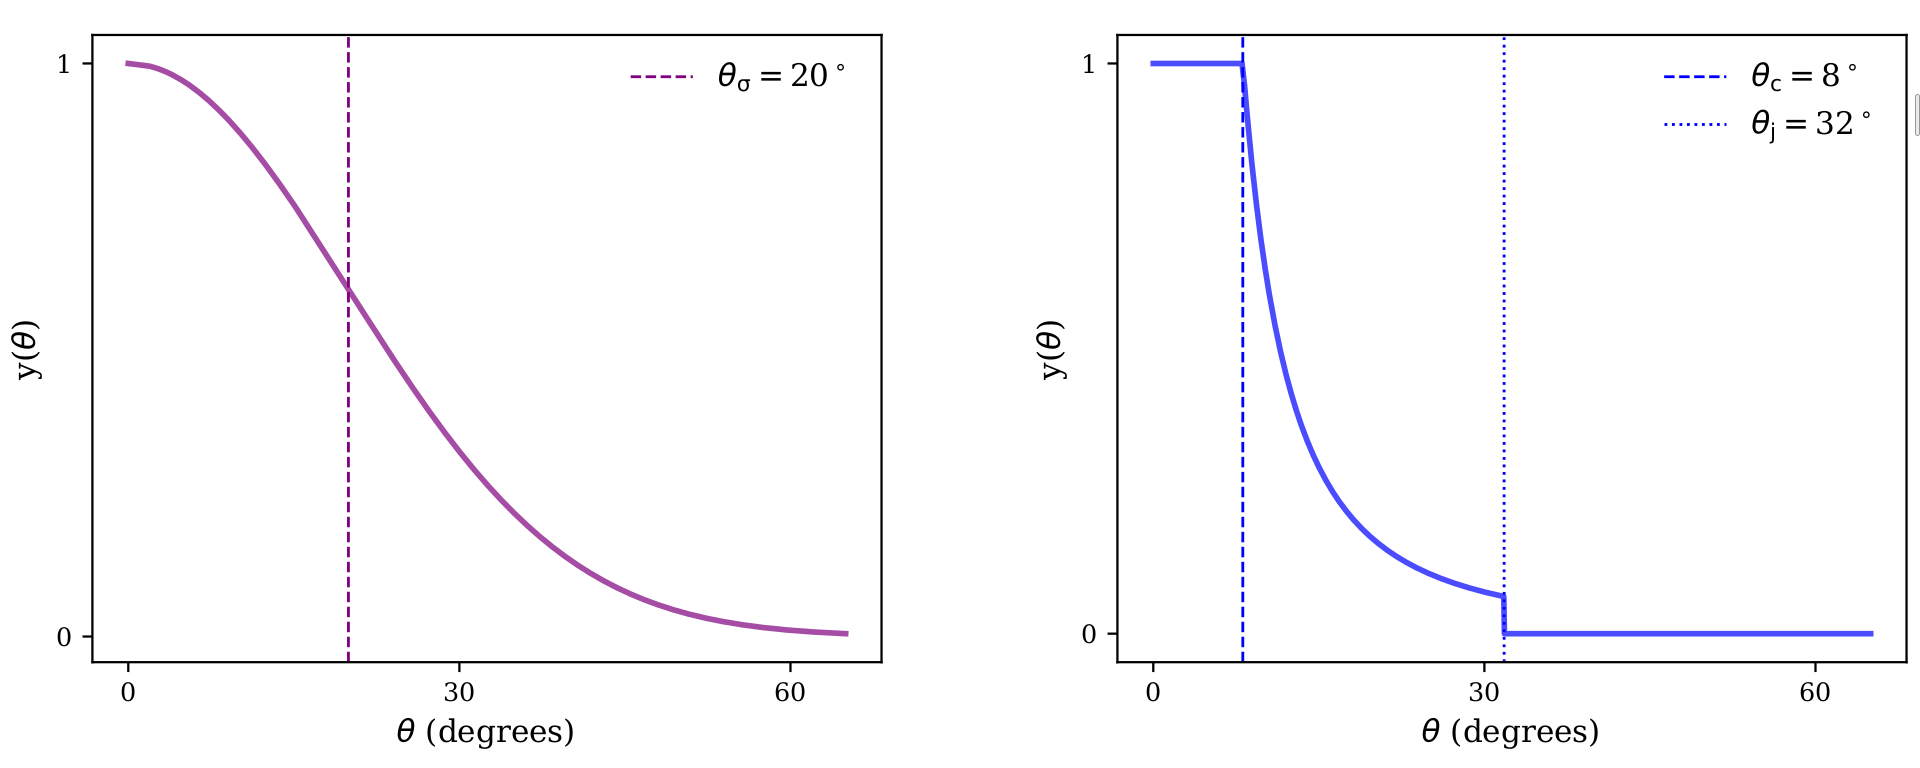
\includegraphics[width=\textwidth]{jet_models}
        \caption[Jet structures as in \cite{hayes_2020}]{
                    Functional forms of the jet structure models, as considered by
                    \cite{hayes_2020}. (Left) The gaussian jet structure with
                    a width $\theta_{\sigma} = 20^{\circ}$, also marked by the dashed
                    line. (Right) The power-law structure with a core angle $\theta_c =
                    8^\circ$ and a jet angle $\theta_j = 32^\circ$.
             }
        \label{fig:jet_models}
    \end{figure}

    In order to compute the observed structure given the intrinsic structure, following
    \cite{granot_2002} we start off by considering the emission profile of a
    point source moving at some angle with the observer, essentially rendering this
    scenario off-axis. This will affect the prompt jet emission, as well as the initial
    afterglow, and so warrants careful analysis.  Now, let the initial jet opening angle
    be $\theta_0$ and let the observer be at an angle $\theta_{obs}$. In general, for a
    point source moving at any angle $\theta$ with respect to the observer, the observed
    flux is given by :

    \begin{equation}
        \label{eq:1}
        F_{\nu} =
           \dfrac{L^{\prime}_{\nu^{\prime}}}{4 \pi d_L^2}
           \left( \dfrac{\nu}{\nu^\prime}\right)^3
                =
            \dfrac{1 + z}{4 \pi d_L^2}
            \dfrac{L^{\prime}_{\nu^{\prime}}}{\gamma^3 (1 - \beta \cos \theta)^3}
    \end{equation}

    Here, $L^{\prime}_{\nu^{\prime}}$ and $\nu^{\prime}$ are the jet comoving frame
    spectral luminosity and frequency, $d_L$ is the luminosity distance, $\gamma = (1 -
    \beta^2)^{-1/2}$ is the jet Lorentz factor. If $t$ and $\nu$ are the observed time
    and frequency  for an observer at $\theta$, and $t_0$ and $\nu_0$ are those for an
    observer on the axis, then:

    \begin{equation}
        \label{eq:2}
        \dfrac{t_0}{t} =
            \dfrac{\nu}{\nu_0}
                       =
            \dfrac{(1 - \beta)}{(1 - \beta \cos \theta)}
            \equiv a
            \approx \dfrac{1}{(1 + \gamma^2 \theta^2)}
    \end{equation}

    And finally putting Eq. \ref{eq:2} into Eq. \ref{eq:1} and expanding using a Taylor
    series approximation upto the leading order:

    \begin{equation}
        \label{eq:3}
        F_{\nu}(\theta_{obs}, t) = a^3 F_{\nu/a}(0, at)
    \end{equation}

    This gives us a handle on how to relate observed off-axis quantities to the on-axis
    ones. Furthermore, this enables us to go from an intrinsic structure to an observed
    one, which is what was required.

\section{Outflows from NSBH Mergers}\label{sec:nsbh}

    The main difference in the NSBH merger pathway to SGRBs, compared to the case of BNS
    mergers, is that though there is theoretical and simulational support for the
    launching of SGRB jets from the merger of a neutron star and a black hole of
    appropriate mass (see for example \cite{ruiz_2020}, \cite{shibata_2019},
    \cite{foucart_2020}), there has not been strong observational evidence for the same.
    In the first half of the third observing run of the LVC (also known as O3a), there
    have been several triggers which have been reportedly confident NSBH triggers.
    However, there were no counterpart EM signals picked up, which decreases the
    credibility of NSBH mergers as the progenitors of SGRBs.\\
    The electromagnetic component from NSBH mergers, is largely decided based on the
    amount of mass left post-merger, outside the horizon of the black hole. This decides
    how much matter participates in the subsequent processes, which may be the rapid
    neutron-capture process which gives rise to the kilonova signal or the magnetic
    field amplification process via the Magneto-Rotational Instability (MRI) which leads
    to a SGRB jet.\\
    Qualitatively, for a binary where the neutron star is treated as a test mass and the
    black hole's spin is aligned with the orbital angular momentum of the binary, the
    innermost-stable circular orbit radius $r_{ISCO}$ scales as $r_{ISCO} \sim
    f(\chi_{BH}) G M_{BH}/c^2$ (where f is a function ranging from 1 to 9, decreasing
    for increasing (prograde) spins; see \cite{bardeen_1972}) and the radius at which
    the tidal disruption of the neutron star occurs, $r_{dis}$ scales as $r_{dis} \sim k
    (M_{BH/M_{BNS}})^{1/3} R_{NS}$ (where k is a constant with a dependence on the black
    hole spin and the equation of state). Only requiring that $r_{dis} \gtrsim
    r_{ISCO}$, as a rough requirement for disruption to occur before the neutron star
    plunges into the black hole, leads to the conclusion that (a.) low-mass black holes
    (b.) larger NS radii (c.) higher prograde black hole spins favour disruption. This
    is seen from Fig. \ref{fig:nsbh_disruption_condition} as well. However, for actual
    quantitative results simulations need to be performed such the effect of the various
    components in the problem are correctly taken into account. As seen from the
    literature, wherein such general-relativistic magnetohydrodynamic simulations are
    carried out, the matter left over post-merger heavily depends on (for a summary, see
    Fig.  \ref{fig:rest_mass_fraction}):

    \begin{itemize}

        \item \textbf{The mass ratio of the system}. This is defined as $q = M_{BH} /
            M_{NS}$ so that $q > 1$ always. Fully general relativistic,
            magnetohydrodynamic simulations (such as \cite{ruiz_2020}) show that in
            cases where the  mass ratio is 3:1, regardless of the neutron spin, a
            collimated outflow is observed, whereas the same is not realised in cases
            where the mass ratio is 5:1 or higher.

        \item \textbf{The spin of the components of the system}. In geometrized units
            (where $G = c = 1$), these are prescribed in terms of $a_{BH} / M_{BH}$ or
            $a_{NS} / M_{NS}$, and whether these two spins align (prograde) or are
            anti-aligned (retrograde) decides whether the neutron star would be tidally
            disrupted, and hence participate in the processes mentioned previously, or
            not. Via simulations, it is seen that the more the prograde spin of the
            neutron star, the farther out the neutron star is tidally disrupted, albeit
            this is only observed for the case of q = 3:1 (comparing say, Figs.
            \ref{fig:nsbh_jet} and \ref{fig:nsbh_5to1}). Also, this leads to long tidal
            tails, which produces a baryon-loaded environment and thus the magnetic
            field of the tidally disrupted matter must overcome the baryon ram pressure
            to launch the jet. This process hence delays the launching of the jet.

    \end{itemize}

    Aside from the SGRB jet, which requires magnetic field amplification (via MRI) as
    well as thermal pair production (from the disk remnant) followed by the
    Blandford-Znajek process, there is a possibility that NSBH mergers can produce
    kilonovae signatures. For this, the dynamically ejected mass has to be between
    $10^{-4.5} - 10^{-2} (M_{NS}/1.4 M_{\odot}) M_{\odot}$ (see \cite{ruiz_2020} for
    more details), and this will lead to kilonovae potentially detectable by the Large
    Synoptic Survey Telescope (LSST).

    \begin{figure}[H]
        \centering
        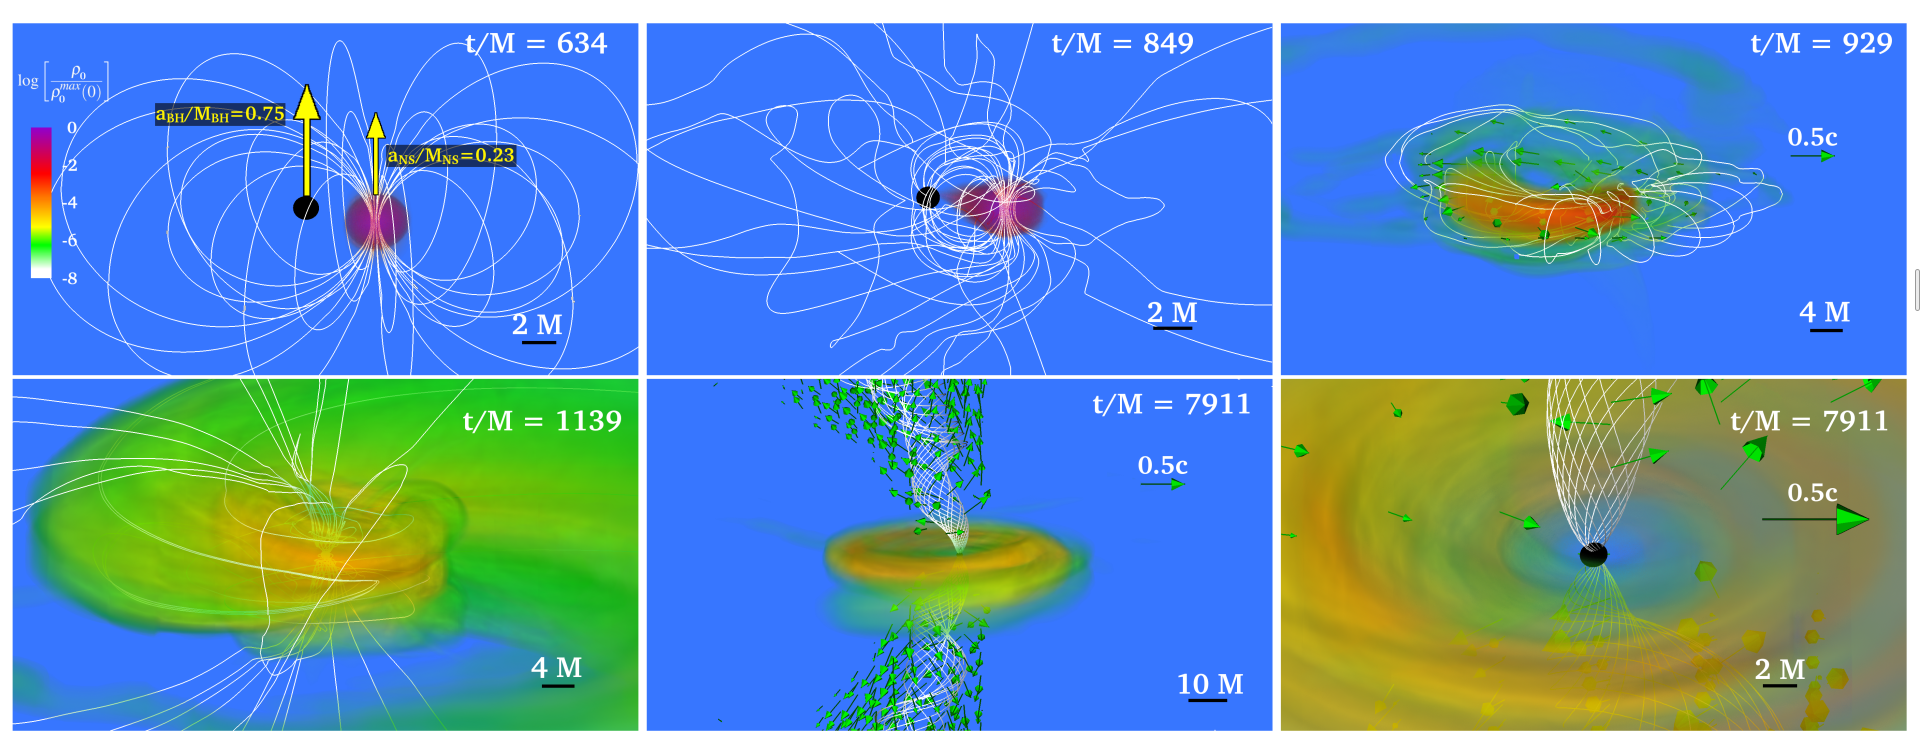
\includegraphics[width=\textwidth]{nsbh_jet}
        \caption[Tidal disruption of a NS in a 3:1 NSBH binary]{
                    Volume rendering of the rest mass density ($\rho_0$) (in log scale),
                    normalized to the NS maximum value $\rho_0 = 8.92 \times 10^{14}
                    (1.4 M_{\odot}/M_{NS})^2 \text{ g/cm}^3$, for particular times for a
                    magnetized neutron star, with q = 3:1 and a prograde NS spin of
                    0.23.  Top three panels highlight the inspiral and the tidal
                    disruption, whereas the bottom three panels highlight the appearance
                    of the magnetically-driven jet. White lines denote the magnetic
                    field, arrows denote the fluid velocity and the BH's apparent
                    horizon is the black sphere. Here M = $2.5 \times 10^{-2}
                    (M_{NS}/M_{1.4M_{\odot}}) \text{ ms} = 7.58
                    (M_{NS}/M_{1.4M_{\odot}}) \text{ km}$ (in geometrized units). From
                    \cite{ruiz_2020}.
             }
        \label{fig:nsbh_jet}
    \end{figure}

    \begin{figure}[H]
        \centering
        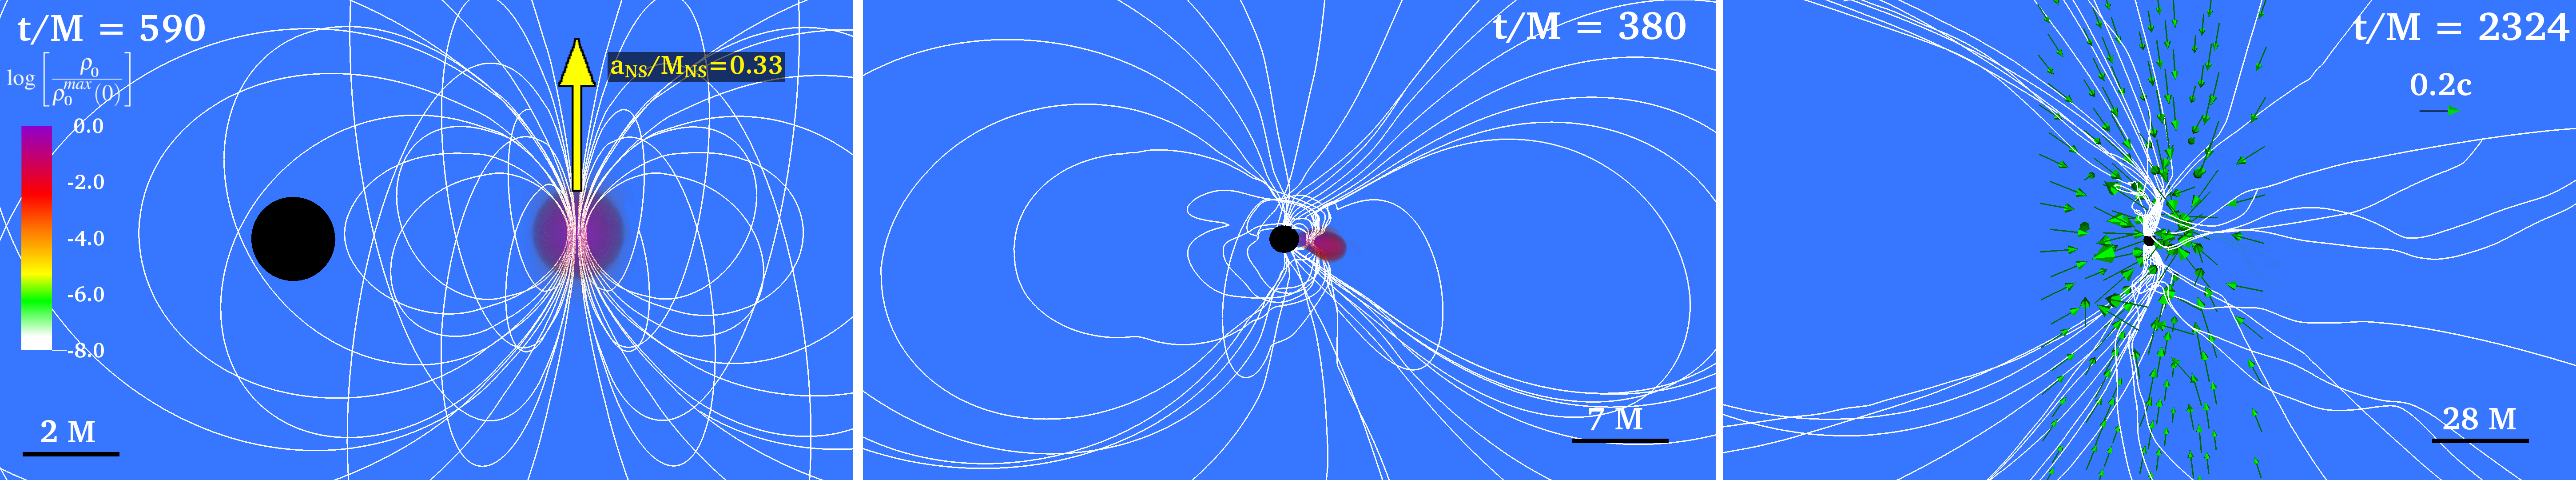
\includegraphics[width=\textwidth]{nsbh_5to1}
        \caption[Tidal disruption of a NS in a 5:1 NSBH binary]{
                    Similar to Fig. \ref{fig:nsbh_jet}, however with the NS spin being
                    0.33, the BH spin being 0 and q = 5:1. In this case, no strong
                    collimation of the magnetic field is observed from the merger
                    remnant, and so a magnetically-driven jet is also not observed.
                    From \cite{ruiz_2020}.
            }
        \label{fig:nsbh_5to1}
    \end{figure}

    \begin{figure}[H]
        \centering
        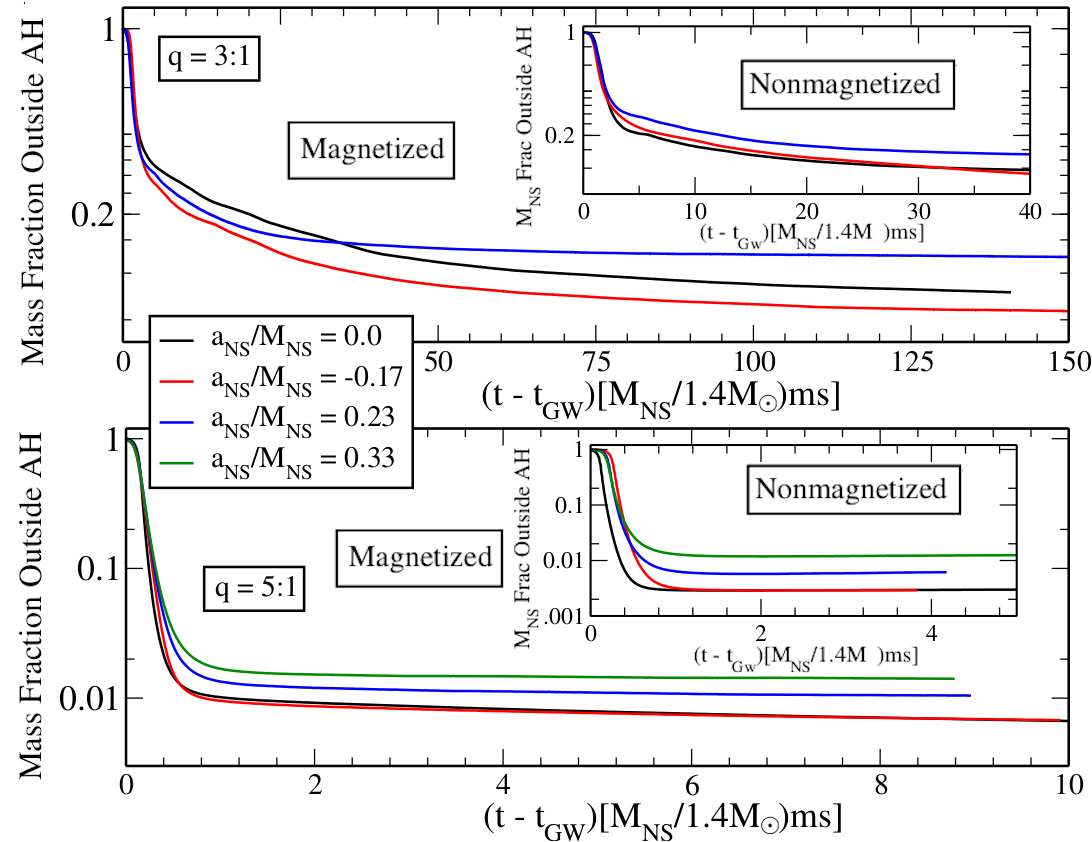
\includegraphics[width=11cm]{rest_mass_fraction}
        \caption[Rest mass outside black hole horizon, as a function of time]{
                    Fraction of rest-mass of the NS outside the apparent horizon of the
                    black hole as a function of coordinate time, for the various
                    configurations considered in \cite{ruiz_2020}. The inset figures
                    report the same for non-magnetized cases, and the coordinate time is
                    shifted such that the merger time coincides with 0.
            }
        \label{fig:rest_mass_fraction}
    \end{figure}

    \begin{figure}[H]
        \centering
        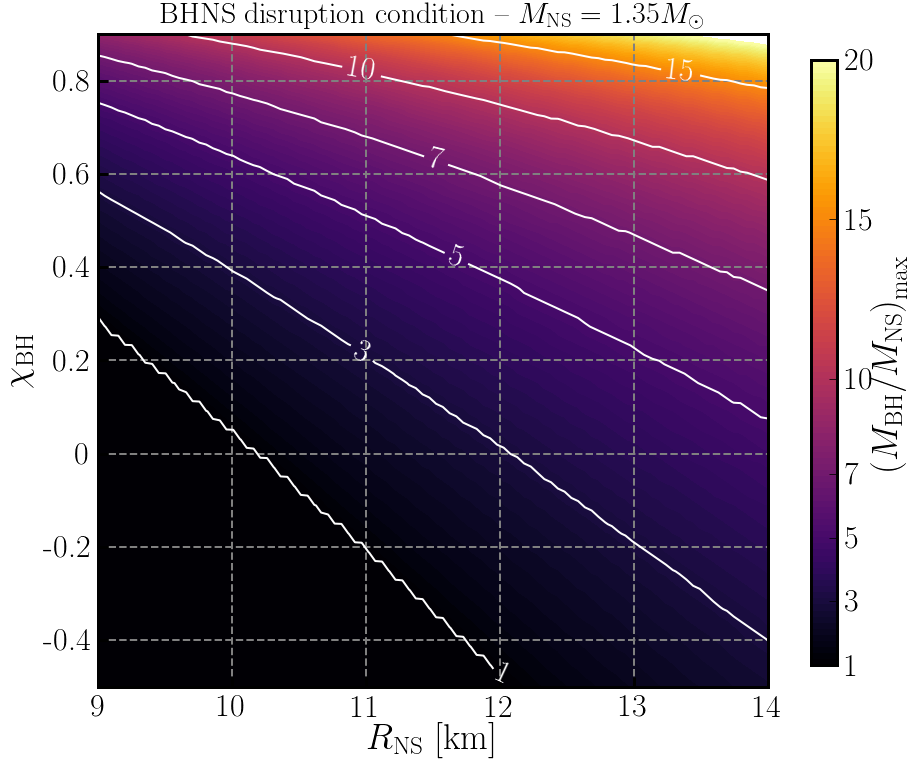
\includegraphics[width=9cm]{nsbh_disruption_condition}
        \caption[Disruption condition in a NSBH binary]{
                    Maximum value of the mass-ratio ($M_{BH}/M_{NS}$) for which a NSBH
                    system disrupts, as a function of the neutron star radius $R_{NS}$,
                    and the aligned component of the dimensionless black hole spin
                    $\chi_{BH}$, assuming $M_{NS} = 1.35 M_{\odot}$. Results for other
                    neutron star masses can be obtained by rescaling considering the
                    disruption condition at constant compaction $C_{NS} = GM_{NS}/R_{NS}
                    c^2$. From \cite{foucart_2020}.
            }
        \label{fig:nsbh_disruption_condition}
    \end{figure}

    \subsection{Modelling outflows from NSBH Mergers}\label{ssec:outflows-nsbh}

    As mentioned before, the outflows from NSBH mergers depend on the amount of mass
    left outside the event horizon post-merger. In the work done by \cite{foucart_2018},
    the authors consider a suite of 75 numerical relativity simulations of NSBH mergers
    over the parameter space $\mathcal{Q} \in [1, 7]$, $ \chi_{BH} \in [-0.5, 0.97]$,
    $\mathcal{C}_{NS} \in [0.13, 0.182]$\footnote{
        Here, $\mathcal{Q} = M_{BH}/M_{NS}$ is the mass-ratio, $\chi_{BH} =
        c|\mathbf{S}|/GM_{BH}^2$ is the effective spin of the black hole and $C_{NS} =
        GM_{NS}/R_{NS}c^2$ is the compactness of the neutron star.
    }
    and fit the results for the \textit{remnant mass} $M_{\mathrm{rem}}$ (sometimes also
    denoted as $M_{\mathrm{out}}$), as a function of the binary parameters (masses,
    spins of the components, tidal deformability of the neutron star etc). This fit is
    given as follows:

    \begin{equation}
        M_{\mathrm{out}} =
            M_{NS}^b \cdot
            \max \left( \alpha \dfrac{1-2\rho}{\eta^{1/3}} -
            \beta \hat{R}_{\mathrm{ISCO}} \dfrac{\rho}{\eta} + \gamma, 0 \right)^\delta
    \end{equation}
    where:

    \begin{itemize}

        \item The baryonic mass of the neutron star is given by the equation $$M_{NS}^b
            = M_{NS} \left(1 + \dfrac{0.6 C_{NS}}{1 + 0.5 C_{NS}} \right)$$

        \item The tidal deformability of the neutron star is given by $\Lambda_{NS}$ and
            $\rho = (15 \Lambda_{NS})^{-1/5}$. It is also related to the compactness of
            the neutron star via the C-Love relation (see \cite{yagi_2017}):
            \begin{equation}
                C_{NS} = \sum_{k=0}^{2} a_k (\ln \Lambda_{NS})^k
            \end{equation}
            where $a_0 = 0.360, a_1 = -0.0335, a_2 = 0.000705$.

        \item $\eta$ is the symmetric mass ratio, given by $ \eta =
            \dfrac{\mathcal{Q}}{(1 + \mathcal{Q})^2} $.

        \item $\hat{R}_{ISCO} = c^2 R_{ISCO} / GM_{BH}$ is the normalized ISCO radius
            for a spinning black hole, given in \cite{bardeen_1972} as :
            \begin{align}
                \begin{split}
                    \hat{R}_{ISCO} &=
                        3 +
                        Z_2 -
                        \mathrm{sgn}(\chi_{BH}) \sqrt{(3 - Z_1)(3+Z_1 + 2Z_2)} \\
                    \hookrightarrow Z_1 &=
                                    1 +
                                    (1 - \chi_{BH}^2)^{1/3}
                                    [(1 + \chi_{BH})^{1/3} + (1 - \chi_{BH})^{1/3}]\\
                    \hookrightarrow Z_2 &=
                                    \sqrt{3\chi_{BH}^2 +  Z_1^2}
                \end{split}
            \end{align}

        \item $(\alpha, \beta, \gamma, \delta) \equiv (0.308, 0.124, 0.283, 1.536)$ are
            the fit coefficients.

    \end{itemize}

    Similarly, \cite{kawaguchi_2016} fit to the results of 45 numerical relativity
    simulations over the parameter space $\mathcal{Q} \in [3,7]$, $\chi_{\mathrm{BH}}
    \in [0, 0.90]$, $C_{\mathrm{NS}} \in [0.138, 0.180]$. This fit produces a formula
    for the \textit{dynamic} mass $M_{\mathrm{dyn}}$, which is the unbound mass ejected
    at the time of disruption, in terms of the binary parameters. This fit is given as
    follows:

    \begin{multline}
        \dfrac{M_{dyn}}{M_{NS}^b} =
            \max \biggl\{
               a_1 Q^{n_1}(1 - 2C_{NS})C^{-1}_{NS} -
               a_2 Q^{n_2} \hat{R}_{ISCO}(\chi_{BH}) + \\
               a_3\left(1 - \dfrac{M_{NS}}{M^b_{NS}}\right) +
               a_4, 0
           \biggr\}
    \end{multline}
    where the symbols have their usual meanings, and additionally:

    \begin{align*}
        a_1 &= 4.464 \times 10^{-2} & a_2 &= 2.269 \times 10^{-3} \\
        a_3 &= 2.431 & a_4 &= -0.4159 \\
        n_1 &= 0.2497 & n_2 &= 1.352
    \end{align*}

    From these two quantities, we can derive the disc mass $M_{\mathrm{disc}}$ as :
    \begin{equation}
        M_{\mathrm{disc}} = \max\{M_{\mathrm{out}} - M_{\mathrm{dyn}}, 0\}
    \end{equation}
    However, due to the fact that these two fits are derived from simulations over
    different regions of the input parameter space, care must be taken while applying
    them together. This is to ensure that $M_{\mathrm{dyn}} \leq M_{\mathrm{out}}$
    always, so that the disc mass is non-negative. This validation is performed by
    considering the ratio $M_{\mathrm{out}} / M_{\mathrm{dyn}}$. Another constraint is
    imposed, which is motivated by the fact that NSBH simulations carried out by
    \cite{foucart_2019} in the near-equal mass ratio regime found an unbound component
    no more massive than roughly 30\% of the total remnant mass (note that one expects
    maximal tidal disruption in this regime, given a fast spinning black hole). Thus we
    set:

    \begin{equation}
        \label{eq:constraint}
        M_{\mathrm{dyn, max}} = f \cdot M_{\mathrm{rem}} = 0.3 \cdot M_{\mathrm{rem}}
    \end{equation}


    Additionally, the masses of the other wind ejecta, namely the neutrino-driven and
    viscosity-driven wind ejecta, are derived from that of the disc mass:
    \begin{align}
        \begin{split}
            M_{\mathrm{vis}} &=
                \xi_{\mathrm{vis}}M_{\mathrm{disc}} =
                    0.2M_{\mathrm{disc}} \\
            M_{\nu} &=
                \xi_{\nu}M_{\mathrm{disc}} =
                    0.01 M_{\mathrm{disc}}
        \end{split}
    \end{align}

    To model the SGRB jet, the procedure of \cite{zhu_2020} is followed. The
    kinetic energy of the jet is decided by the disc mass and the black hole spin as
    follows:
    \begin{equation}
        E_{\mathrm{K, jet}} =
            \epsilon(1 - \xi_{\mathrm{vis}} - \xi_{\nu})
            M_{\mathrm{disc}} c^2 \Omega_H^2 f(\Omega_H)
        \label{eq:e_kin_jet}
    \end{equation}
    where:

    \begin{itemize}

        \item The dimensionless angular velocity at the horizon of the black hole is
            given by:
            \begin{equation}
                \Omega_H = \dfrac{\chi_{BH}}{2(1 + \sqrt{1 + \chi_{BH}^2}}
            \end{equation}

        \item $f(\Omega_H)$ is a high-spin correction factor given by:
            \begin{equation}
               f(\Omega_H) = 1 + 1.38\Omega_H^2 - 9.2 \Omega_H^4
               \label{eq:Omega_h}
            \end{equation}
        \item $\epsilon$ is a fudge factor which depends on the large-scale geometry of
            the magnetic field, disc aspect ratio and the ratio of the magnetic field
            energy density to disc pressure at saturation.\\ In order to set it to a
            definite value, it is noted that the maximum disc mass cannot exceed the
            total NS baryonic mass i.e. $M_{\mathrm{disc}} \lesssim 2M_\odot$. Also, the
            spin-dependent factor $\Omega_H^2f(\Omega_H)$ cannot exceed 0.2 (since
            $\chi_{BH} \in [-1, 1]$). Furthermore, the most energetic of SGRBs has had a
            $E_{\gamma, \mathrm{iso}} \sim 7.4 \times 10^{52}$ erg, and if one assumes a
            10\% conversion efficiency of kinetic to gamma-ray energy alongwith a
            typical jet opening angle of 5$^{\circ}$, this corresponds to a kinetic
            energy of $E_{\mathrm{K, jet}} \sim 3 \times 10^{52}$ erg.\\
            Based on this, once can calculate $\boxed{\epsilon \approx 0.015}$.

    \end{itemize}

    Using this we can define the structure of the SGRB jet, given by the following
    equations:

    \begin{equation}
        \dfrac{dE(\theta)}{d\Omega} =
            \dfrac{E_{\mathrm{k, jet}}}{\pi \theta_{\mathrm{c, E}}^2}
            e^{-(\theta/\theta_{\mathrm{c, E}})^2}
        \label{eq:dE_dOmega}
    \end{equation}

    \begin{equation}
        \Gamma(\theta) = (\Gamma_c - 1)e^{-(\theta/\theta_{\mathrm{c, E}})^2} + 1
    \end{equation}

    \begin{equation}
        E_{\mathrm{iso}}(\theta_v) =
            \eta \int \dfrac{\delta^3}{\Gamma} \dfrac{dE}{d\Omega} d\Omega
        \label{eq:eiso}
    \end{equation}
    where:

    \begin{itemize}

        \item $\Gamma_c = 100, \theta_{\mathrm{c, E}} = 0.1, \theta_{\mathrm{c}, \Gamma}
            = 0.2$.  See \cite{salafia_2015} and \cite{barbieri_2019}.

        \item $\eta$ is the conversion efficiency of gamma-ray energy to kinetic energy,
            which is traditionally taken to be 10\%.

        \item $\delta$ is the Doppler factor, given by $$\delta = \dfrac{1}{\Gamma[1 -
            \beta \cos \alpha_v]}$$ where $\alpha_v$ is the angle between the jet
            element at $(\theta, \phi)$ and the observer's direction.
    \end{itemize}

\section{NS mergers in GW regime}

    Consider any astrophysical source emitting gravitational waves, which come in two
    polarizations, namely the \emph{plus} $h_{+}(t; \mathbf{\Theta}_{GW})$ and the
    \emph{cross} $h_{\times}(t; \mathbf{\Theta}_{GW})$ polarizations. Here
    $\mathbf{\Theta}_{GW}$ is the parameter vector, and is typically $\{m_1, m_2,
    \mathbf{\chi}_1, \mathbf{\chi}_2, D_L, \iota, t_c, \phi_c\}$ which are the component
    masses, component spins, the binary's luminosity distance, the inclination angle
    of the orbital plane with respect to the line of sight, and two constants of
    integration: the time and phase of coalescence.\\
    A detector's response is recorded as the GW strain such waveforms produce, but in
    the frequency domain and so the input waveforms are Fourier transformed before
    processing. Also the detector's antenna patterns (sensitivity as a function of the
    source location on the sky) and location phase factor (effect of the earth's
    rotation) play a role in the response. Thus, the detector response to these
    gravitational waves is of the form:
    \begin{equation}
        H(f; \mathbf{\Theta}) =
            F_{lp}(f; \alpha, \delta) \cdot
            [
                H_{+}(f; \mathbf{\Theta}_{GW}) F_{+}(f; \alpha, \delta, \psi) +
                H_{\times}(f; \mathbf{\Theta}_{GW}) F_{\times}(f; \alpha, \delta, \psi)
            ]
    \end{equation}
    where $F_{lp}$ is the location phase factor as a function of the frequency and the
    source RA and declination, $H_{+/\times}$ are the frequency domain waveforms, and
    $F_{+/\times}$ are the detector antenna patterns for each polarization. Also
    $\mathbf{\Theta} = \{\mathbf{\Theta}_{GW}, \alpha, \delta, \psi\}$.\\
    The sensitivity of a detector is given by the detector's noise $n(t)$ and its
    autocorrelation $\kappa = \overline{n(t_1)n(t_2)}$. Usually, the noise is assumed to
    be stationary, zero-mean and Gaussian. Thus, one can define the one-sided power
    spectral density $S_n(f)$ as the Fourier transform of the autocorrelation.\\
    From this, one can define the `overlap' between two GW signals (for eg.: the
    detector responses for two different waveforms) using the noise-weighted scalar
    product:
    \begin{equation}
        \langle H, G \rangle =
            2 \int_{0}^{\infty} \dfrac{H(f)G^{\ast}(f) + H^{\ast}(f)G(f)}{S_n(f)} df
    \end{equation}
    And using this definition of the scalar product, the signal-to-noise ratio is
    defined as :
    \begin{equation}
        \rho^2 =
            \langle H, H \rangle =
                4 \int_0^\infty \dfrac{|H(f)|^2}{S_n(f)} df
    \end{equation}
    Now, since the noise $n(t) = s(t) - h(t)$ is assumed to a zero-mean Gaussian, its
    Fourier transform also behaves the same way, and thus the probability of noise can
    be written down as :
    \begin{equation}
        \label{eq:probability}
        p(\mathbf{\Theta}) =
            p^0(\mathbf{\Theta})
            e^{
                -\frac{1}{2}
                \langle S - H(\mathbf{\Theta}), S - H(\mathbf{\Theta}) \rangle
            }
    \end{equation}
    where $p^0$ is the prior on the parameter vector of the detector response. Assuming
    that an event signal S has a high SNR, the value of $\mathbf{\Theta}$ at peak
    probability is a good estimate of the true value $\mathbf{\Theta}^{\ast}$.
    Additionally peak probability occurs when the exponential $E = \langle S - H, S - H
    \rangle$ is the largest. Expanding it around the maximum value:
    \begin{equation}
        E(\mathbf{\Theta}) =
            E(\mathbf{\Theta}^{\ast}) +
            \dfrac{1}{2}
            \dfrac{\partial^2 E(\mathbf{\Theta})}{\partial \Theta_i \partial \Theta_j}
            \bigg\rvert_{\mathbf{\Theta} =
                \mathbf{\Theta}^{\ast}}
                \Delta\Theta_i \Delta\Theta_j +
                \cdots
    \end{equation}
    where $\Delta \Theta_i = \Theta_i - \Theta_i^\ast$. The Hessian given by:
    \begin{equation}
        \dfrac{\partial^2 E(\mathbf{\Theta})}{\partial \Theta_i \partial \Theta_j} =
            2 \langle
                  \partial_{\Theta_i} H(\mathbf{\Theta}),
                  \partial_{\Theta_j} H(\mathbf{\Theta})
              \rangle +
              \langle
                  \partial_{\Theta_i} \partial_{\Theta_j} H(\mathbf{\Theta}),
                  N
              \rangle
    \end{equation}
    can be simplified for large SNR, where second-order differentials become negligible.
    This leads to the definition of the Fisher Information Matrix $\Gamma$:
    \begin{equation}
        \Gamma_{ij} =
            \langle
                \partial_{\Theta_i} H(\mathbf{\Theta}),
                \partial_{\Theta_j} H(\mathbf{\Theta})
            \rangle
    \end{equation}
    And hence, Eqn. \ref{eq:probability} becomes:
    \begin{equation}
        p(\mathbf{\Theta}) \sim
            \exp\left(
                         -\dfrac{1}{2}
                          \Gamma_{ij}
                          \Delta\Theta_i
                          \Delta\Theta_j
                \right)
    \end{equation}
    which implies that the assumption of Gaussian noise helps associate the FIM to the
    inverse of the covariance matrix $\Sigma \equiv \Gamma^{-1}$. This also means that
    the diagonal and off-diagonal elements of $\Gamma^{-1}$ denote the variances and
    covariances of the parameters, respectively, with 1$\sigma$ estimates of the error
    are given as $\sigma_{\Theta_i} = \sqrt{\Sigma_{ii}}$.\\
    This Fisher Information Matrix (FIM) formalism\footnote{
        Sometimes also referred to as the Fisher Information Formalism (FIF), in which
        case the Fisher information is not a matrix but is instead the variance of the
        partial derivative with respect to the parameter vector, of the natural
        logarithm of the likelihood function for the random variable whose parameters
        are to be estimated.
    } is a method of rapid GW data analysis, which approaches the accuracy of
    traditional Bayesian parameter estimation for events with large SNR.\\
    \textbf{GWBENCH} (see \cite{borhanian_2020}) is a GW benchmarking tool, which can
    compute the Fisher matrix for a particular NS merger, given the network
    configuration and binary parameters. In this way, it enables rapid calculations to
    benchmark detector upgrades as well as forecast the confidence with which parameters
    may be estimated for the NS mergers in question.\\

\section{Summary}

    NS mergers can present an ideal testing environment for physical theories under
    extreme gravity, and by observing them in both the EM and GW windows, current
    theories can be better understood and refined. Several questions also remain about
    the exact mechanisms which power the outflows from these NS mergers.\\
    In this report, we focus mainly on SGRB jets from NSBH mergers and perform
    population synthesis studies to infer the conditions for and implications of
    observing a SGRB jet from NSBH mergers.
